\documentclass[12pt, oneside]{book}
% This provides the \BibTeX macro
\usepackage{doc}
\usepackage{makeidx}
\usepackage[tight,footnotesize]{subfigure}
\usepackage{amsmath}
\usepackage{amsfonts}
\newtheorem{problem}{Problem}
\newtheorem{definition}{Definition}
\usepackage{graphicx}
\graphicspath{{./figs/}}
%\usepackage{algorithmic}
\usepackage{listings}
\usepackage[noend]{algpseudocode}
\usepackage{hyperref}
\hypersetup{
    colorlinks,
    citecolor=black,
    filecolor=black,
    linkcolor=black,
    urlcolor=black
}
\usepackage{color}
\definecolor{lightgray}{rgb}{.9,.9,.9}
\definecolor{darkgray}{rgb}{.4,.4,.4}
\definecolor{purple}{rgb}{0.65, 0.12, 0.82}
\lstdefinelanguage{JavaScript}{
  keywords={typeof, new, true, false, catch, function, return, null, catch, switch, var, if, in, while, do, else, case, break},
  keywordstyle=\color{blue}\bfseries,
  ndkeywords={class, export, boolean, throw, implements, import, this},
  ndkeywordstyle=\color{darkgray}\bfseries,
  identifierstyle=\color{black},
  sensitive=false,
  comment=[l]{//},
  morecomment=[s]{/*}{*/},
  commentstyle=\color{purple}\ttfamily,
  stringstyle=\color{red}\ttfamily,
  morestring=[b]',
  morestring=[b]"
}

\lstset{
   language=JavaScript,
   backgroundcolor=\color{lightgray},
   extendedchars=true,
   basicstyle=\footnotesize\ttfamily,
   showstringspaces=false,
   showspaces=false,
   numbers=left,
   numberstyle=\footnotesize,
   numbersep=9pt,
   tabsize=2,
   breaklines=true,
   showtabs=false,
   captionpos=b
}

\newcommand{\setR}{\ensuremath{\mathbb{R}}}
\newcommand{\col}{\ensuremath{c}}
\newcommand{\row}{\ensuremath{r}}
\newcommand{\R}{\ensuremath{\field{R}}}
\newcommand{\sparsifysymbol}{\ensuremath{\rho}}
\newcommand{\sparsify}[1]{\ensuremath{\sparsifysymbol(#1)}}
\newcommand{\todo}[1]{\textbf{#1}}
\newcommand{\nnz}[1]{\ensuremath{\operatorname{nz}(#1)}}
% Define the name of the two minimization problems
\newcommand{\MinStaBic}{\textsc{MinimumStarBicoloring}}
\newcommand{\MinUniCom}{\textsc{MinimumUnidirectionalCompression}}
\newcommand{\MinBidCom}{\textsc{MinimumBidirectionalCompression}}

\begin{document}
\begin{center}
\begin{minipage}{0.75\linewidth}
    \centering
    
\includegraphics[width=0.3\linewidth]{logo}
    \par
    \vspace{3cm}
    {\uppercase{\Large Preconditioning\par}}
    \vspace{3cm}
    {\Large Mohammad Ali Rostami\par}
    \vspace{3cm}
    {\Large Supervisor: Prof. Martin B{\"u}cker\par}
    \vspace{3cm}
    {\Large January 2016}
\end{minipage}
\end{center}
\clearpage

\newpage
\section*{Abstract}

\thispagestyle{empty}

\newpage
\section*{Acknowledgments}
\thispagestyle{empty}

\tableofcontents

\chapter{Introduction}
Partial differential equations (PDE) are the most common models of the real-world problems.
Iterative solvers are a solution to these linear systems which need a multiplication
 of Jacobian and a vector in each iteration. 
Many strategies were studied to compute these products efficiently.
Automatic Differentiation~\cite{Griewank2008EDP,Rall1981ADT} 
computes not only the differentiation wtihout numerical errors but also the
matrix-vector multiplication automatically. 
Based on this ability of AD techniques, different methods are analysed to 
reduce the memory that is needed to store the Jacobian matrix as well as
speeding up the computation. These methods are generally as a part of 
a bigger area called combinatorial scientific computing.

In this work, we discuss an interactive educational tool and a computational package 
for coloring for the area of combinatorial scientific computing.
So, we discuss the basic concepts needed throughout this work in Chapter~\ref{prel}.
Then, we visualize different algorithms from this area in Chapter~\ref{explain}.
The computational package for coloring is discussed later in Chapter~\ref{package}.
Implementation details and conculsion comes at the end in Chapters~\ref{impl} and
~\ref{conc}.



\chapter{Preliminaries}
\label{prel}
We will discuss AD and the needed seed matrices in~\ref{s.seedmatrix} which is based on
our paper~\cite{2014:09}.
%===================================================================================================
\section{Jacobian Computation}
\label{s.seedmatrix}
%===================================================================================================
Given a program to evaluate some function $f(x) : \setR^n \rightarrow \setR^m$,
techniques of automatic differentiation (AD)~\cite{Griewank2008EDP,Rall1981ADT} generate
computer programs capable of evaluating the $m \times n$ Jacobian matrix $J$. In the
\emph{forward mode} (FM) of AD, the automatically-generated program computes the product
$JV$; in the \emph{reverse mode}, it computes the product $WJ$. In these matrix-matrix
products, the two binary input matrices $V \in \{0,1\}^{n\times \col}$ and $W\in
\{0,1\}^{\row\times m}$ are called \emph{seed matrices}. The products $JV$ and $WJ$ are
computed without assembling the Jacobian $J$. Compared to the time needed to evaluate
$f(x)$, the computational cost of computing $JV$ in the forward mode is larger by a
factor of \col, the number of columns of $V$. The corresponding factor for the reverse
mode to compute $WJ$ is given by \row, the number of rows of $W$.

In general, the Jacobian $J$ is computed choosing either $c=n$ and $V$ as the identity of
order~$n$ in the forward mode or $r = m$ and $W$ as the identity of order $m$ in the
reverse mode. However, if $J$ is sparse and its sparsity pattern is known the number of
columns of~$V$ in the forward mode or the number of rows of~$W$ in the reverse mode can
be reduced to $\col < n$ or $\row < m$ such that all nonzero entries of $J$ still appear
in the product $JV$ or $WJ$. This way, the computational cost is decreased using either
the forward mode with a suitable linear combination of the columns of~$J$ or the reverse
mode with a suitable linear combination of the rows of~$J$; see the
survey~\cite{Gebremedhin05whatcolor}.

The key idea behind this \emph{unidirectional compression} is now illustrated for the
forward mode. Let $J=[c_1, c_2, \dots, c_n]$ denote the Jacobian matrix whose $i$th
column is represented by the vector $c_i \in \setR^m$. Two columns $c_i$ and $c_j$ are
called \emph{structurally orthogonal} if they do not have any nonzero element in a same
row. Two columns are called \emph{structurally non-orthogonal} if there is at least one
row in which both columns, $c_i$ and $c_j$, have a nonzero element. The number of columns
of the seed matrix is then reduced by forming linear combinations of structurally
orthogonal columns. More precisely, a set $S$ of structurally orthogonal columns can be
represented by a single column of the product $JV$ because the sum of these columns
contains all the nonzero entries of all the columns in $S$. Analogously, two rows are
\emph{structurally orthogonal} if they do not have any nonzero element in a same column.
A set of structurally orthogonal rows is represented by a single row in the product $WJ$.
The computational cost then scales with the number of groups of structurally orthogonal
columns or rows in the forward or reverse mode, respectively.

To illustrate this, we consider the following three $6 \times 6$ Jacobian matrices:
\begin{equation*}
A =
 \begin{bmatrix}
 1  & 0 & 0 & 0 & 0 & 0 \\
 2  & 7 & 0 & 0 & 0 & 0 \\
 3  & 0 & 8 & 0 & 0 & 0 \\
 4  & 0 & 0 & 9 & 0 & 0 \\
 5  & 0 & 0 & 0 & 10& 0 \\
 6  & 0 & 0 & 0 & 0 & 11
 \end{bmatrix}, \;\,
B =
 \begin{bmatrix}
 1  & 2 & 3 & 4 & 5 & 6 \\
 0  & 7 & 0 & 0 & 0 & 0 \\
 0  & 0 & 8 & 0 & 0 & 0 \\
 0  & 0 & 0 & 9 & 0 & 0 \\
 0  & 0 & 0 & 0 & 10& 0 \\
 0  & 0 & 0 & 0 & 0 & 11
 \end{bmatrix}, \;\,
 %
 C =
  \begin{bmatrix}
 1  & 7  & 8  & 9  & 10 & 11 \\
 2  & 12 & 0  & 0  & 0  & 0 \\
 3  & 0  & 13 & 0  & 0  & 0 \\
 4  & 0  & 0  & 14 & 0  & 0 \\
 5  & 0  & 0  & 0  & 15 & 0 \\
 6  & 0  & 0  & 0  & 0  & 16
 \end{bmatrix}.
\end{equation*}
Since all elements of column $1$ of $A$ are nonzero, this column is not structurally
orthogonal to any of the other columns. Similarly, row $1$ of $B$ is not structurally
orthogonal to any of the other rows. However, the columns $2$, $3$, $4$, $5$, and $6$ of
the matrix $A$ are structurally orthogonal and so are rows $2$, $3$, $4$, $5$, and $6$
of~$B$. Therefore, we build two groups, $\{1 \}$ and $\{2, 3, 4, 5, 6\}$, of structurally
orthogonal columns of $A$ as well as two groups, $\{1 \}$ and $\{2, 3, 4, 5, 6\}$, of
structurally orthogonal rows of $B$. This grouping of structurally orthogonal columns and
rows is represented by the two seed matrices and their resulting matrix-matrix products:
$$
V =
\begin{bmatrix}
 1  & 0 \\
 0  & 1 \\
 0  & 1 \\
 0  & 1 \\
 0  & 1 \\
 0  & 1
\end{bmatrix},\;\,
%
AV =
\begin{bmatrix}
 1  & 0 \\
 2  & 7 \\
 3  & 8 \\
 4  & 9 \\
 5  & 10\\
 6  & 11
\end{bmatrix}
\qquad\text{and}\qquad
\begin{aligned}
  W &=
    \begin{bmatrix}
     1  & 0 & 0 & 0 & 0 & 0\\
     0  & 1 & 1 & 1 & 1 & 1\\
    \end{bmatrix}, \\[1em]
  %
  WB &=
     \begin{bmatrix}
      1  & 2 & 3 & 4 & 5 & 6\\
      0  & 7 & 8 & 9 & 10 & 11
     \end{bmatrix}.
\end{aligned}
$$
Each group of structurally orthogonal columns of $A$ corresponds to a column in the seed
matrix~$V$. Similarly, each group of structurally orthogonal rows of $B$ corresponds to a
row in the seed matrix $W$. All nonzero elements of $A$ also appear in $AV$ and all
nonzero elements of $B$ also appear in $WB$. The computational cost using either the
forward mode or the reverse mode is decreased from taking identity seed matrices of order
$n=m=6$ to seed matrices $V$ and $W$ with $\col = \row = 2$, representing two groups of
structurally orthogonal columns/rows.

Next, consider the matrix $C$ that has neither structurally orthogonal columns nor
structurally orthogonal rows. Therefore, there is no unidirectional compression of the
matrix $C$, neither by \col\ columns nor by \row\ rows, that reduce \col\ or \row\ below
$n = m = 6$. However, a linear combination of both, columns and rows, can be used to
reduce the computational cost to a value below six. Here, the columns and rows of a
corresponding group are not necessarily structurally orthogonal. This technique in which
the forward and reverse mode are used in a combined way is called \emph{bidirectional
compression}. There are various ways to carry out this compression. One option for this
example is to choose
\begin{equation}
\label{e.onesvw}
V =
\begin{bmatrix}
 1  & 0\\
 0  & 1 \\
 0  & 1 \\
 0  & 1 \\
 0  & 1\\
 0  & 1
\end{bmatrix},\;\,
%
CV =
\begin{bmatrix}
 1  & 45\\
 2  & 12 \\
 3  & 13 \\
 4  & 14 \\
 5  & 15\\
 6  & 16
\end{bmatrix}
\qquad\text{and}\qquad
\begin{aligned}
  W &=
   \begin{bmatrix}
    1  & 0 & 0 & 0 & 0 & 0\\
   \end{bmatrix}, \\[1em]
  WC &=
   \begin{bmatrix}
    1  & 7 & 8 & 9 & 10 & 11
   \end{bmatrix}.
\end{aligned}
\end{equation}
All nonzero elements of $C$ also appear in the pair~$CV$ and $WC$. Notice that the
nonzero element~$1$ is contained in both products and that the product $CV$ contains the
value~$45$ which is irrelevant to compute all nonzero elements of $C$. The computational
cost of a bidirectional compression is dominated by the sum of the costs of the forward
and reverse mode which is $\col + \row = 3$ in this example. By counting the occurrences
of ones in the seed matrices in \eqref{e.onesvw}, we see that 6 columns, but only a
single row of $C$ are used to form the groups of columns/rows. In general, it is
sufficient to form these groups by choosing subsets of the columns and rows of a given
sparse matrix.

The above example is intentionally kept simple. However, for general sparsity patterns,
it is not always easy to figure out how to linearly combine columns and rows such that
the computational cost is minimized. Hence, we introduce the following combinatorial
optimization problems that addresses this question of unidirectional or bidirectional compression. 
In practice, the solution of this
problem will substantially reduce the computational cost for computing all nonzero
elements of a large and sparse Jacobian.

\begin{problem}[\MinUniCom]
\label{p.seed.uni} Let $J$ be a sparse ${m\times n}$ Jacobian matrix with known sparsity
pattern. Find a seed matrix $V$ of dimension $n\times \col$ 
whose number of columns of $V$ sums up
to a minimal value, $\col$, such that all nonzero elements of $J$ also appear in
the matrix-matrix product $JV$.
\end{problem}

\begin{problem}[\MinBidCom]
\label{p.seed.bid} Let $J$ be a sparse ${m\times n}$ Jacobian matrix with known sparsity
pattern. Find a pair of binary seed matrices $V$ of dimension $n\times \col$ and $W$~of
dimension $\row \times m$ whose number of columns of $V$ and number of rows of $W$ sum up
to a minimal value, $\col + \row$, such that all nonzero elements of $J$ also appear in
the pair of matrix-matrix products $JV$ and $WJ$.
\end{problem}

An equivalent graph-theoretical formulation of this problem is discussed in the next
section.

%==========================================================================================
\section{Combinatorial Model}
\label{s.modeling}
%==========================================================================================
Graph models are ubiquitous in exploiting the sparsity involved in derivative
computations; see the comprehensive survey \cite{Gebremedhin05whatcolor}. In the context of the
semi-matrix-free approach introduced in the previous section, the discussion is based on
the following undirected graph model.
%
\begin{definition}[Column Intersection Graph]
\label{d:cig}
The column intersection graph $G = (V,E)$ associated with an $n \times n$ Jacobian $J$
consists of a set of vertices $V=\{v_1, v_2, \dots, v_n\}$ whose vertex $v_i$ represents
the $i$th column $J(:,i)$. Furthermore, there is an edge $(v_i,v_j)$ in the set of edges
$E$ if and only if the columns $J(:,i)$ and $J(:,j)$ represented by $v_i$ and $v_j$ have
a nonzero element in at least a same row position.
\end{definition}

The grouping of columns is encoded in the following definition.
%
\begin{definition}[Coloring]
A coloring of $G$ is a mapping $\Phi : V \to {1, \dots, p}$ with the property
$\Phi(v_i)\neq \Phi(v_j)$ for $(v_i,v_j) \in E$.
\end{definition}
%
Coleman and Mor\'{e} \cite{Coleman1983EoS} then showed that Problem~\ref{p.seed.uni}, which
asks for a seed matrix with a minimal number of columns, is equivalent to the following
coloring problem.
%
\begin{problem}[Minimum Coloring]
\label{p:mincol}
%
Find a coloring $\Phi$ of the column intersection graph $G$ with a minimal number of
colors.
\end{problem}

The intimate connection between the sparse Jacobian computations described in
Problem~\ref{p.seed.uni} and the graph coloring issues described by Problem~\ref{p:mincol} is
well-known.
We illustrated this algorithm by an interactive educational module EXPLAIN~\cite{2013:05}
(see Section~\ref{s.column-compression}). 

This undirected graph model is easily adapted to unidirectional compression with respect
to rows. Here, a vertex represents a row and an edge represents structural
non-orthogonality of two rows. However, the undirected graph model is not sufficient to
capture the properties involved in bidirectional compression. An obvious reason is that,
for a rectangular Jacobian matrix, a bidirectional compression requires to model columns
and rows separately. It is therefore common to consider a bipartite graph
model~\cite{Coleman1996SaE,cv:ecs,hs:csj}. In this model, the vertex set $V=V_c\cup V_r$
is decomposed into a set of vertices~$V_c$ representing columns of $J$ and another set of
vertices~$V_r$ representing rows. The set of edges~$E$ is used to represent the nonzero
elements and it is defined as follows. An edge $(c_i , r_j) \in E$ connects a column
vertex $c_i \in V_c$ and a row vertex $r_j \in V_r$ if there is a nonzero element in $J$
at the position represented by $c_i$ and $r_j$. The graph is bipartite indicating that
all edges connect vertices from one set~$V_c$ to the other set $V_r$. That is, there is
no edge connecting vertices within the set $V_c$ or within $V_r$. Moreover, two vertices
that are connected by a path of length two, are called \emph{distance-$2$ neighbors}.

The overall idea behind transforming Problem \ref{p.seed.bid}, \MinBidCom, into an equivalent
problem using the bipartite graph model is as follows. The grouping of the columns and
rows is expressed by representing each group by a color. Vertices that belong to the same
group of columns/rows are assigned the same color. Formally, this is represented by a
coloring of a bipartite graph. Such a coloring is mapping
$$
\Phi:V_c \cup V_r \to \{0,1,\dots ,p\}
$$
that assigns to each vertex a color represented by an integer. Recall from the previous
section that, in general, there can be columns or rows that are not chosen in the
grouping at all. Therefore, the coloring~$\Phi$ also involves a ``neutral'' color
representing this ``don't color'' situation. A vertex $v \in V_c \cup V_r$ that is not
used in the grouping of columns/rows is assigned the neutral color $\Phi(v)=0$. More
precisely, if $\Phi(v)=0$ for a column vertex $v$ then every nonzero represented by an
incident edge of $v$ is determined by a linear combination of rows. Similarly, a nonzero
entry represented by an edge that is incident to a neutrally-colored row vertex is
determined by a linear combination of columns.

To represent the process of finding seed matrices using the bipartite graph model, it is
necessary to consider the underlying properties, which are as follows:
\begin{enumerate}
\item The computational cost roughly consists of the number of groups of columns and
    rows. Since the overall cost is the sum of the costs associated to the forward mode
    and to the reverse mode, the (non-neutral) colors for the forward mode and the
    (non-neutral) colors for the reverse mode need to be different.

\item Recall from our example with the products $CV$ and $WC$ that some nonzero
    elements may be computed twice, by the forward mode in $JV$ and by the reverse mode
    in $WJ$. Therefore, an edge representing such a nonzero element connects two
    vertices with two different non-neutral colors. In general, since problem
    \MinBidCom\ asks for computing \emph{all} nonzero elements, at least one vertex of
    every edge has to be colored with a non-neutral color.

\item Recall from the example that structural orthogonality is no longer required for
    grouping the rows and columns. However, there is still the following restriction.
    Suppose two columns are structurally non-orthogonal and have a nonzero element in a
    same row. If this row is not handled by the reverse mode, these two columns need to
    be in different column groups. The same argument holds for corresponding situations
    with row groups.

\item Consider three nonzero elements in matrix positions $(i,k)$, $(i,\ell)$, and
    $(j,k)$. Suppose that the nonzero at $(i,k)$ is computed by the reverse mode
    assigning some (non-neutral) color to the row vertex $r_i$. Then, if $(j,k)$ is
    also computed via the reverse mode, a second (non-neutral) color is needed for
    $r_j$. Now, if $(i,\ell)$ is already determined by the reverse mode for row $i$ the
    column vertex $c_\ell$ is assigned the neutral color. However, if $(i,\ell)$ is
    computed by the forward mode, a third (non-neutral) color is needed for $c_\ell$. A
    similar argument holds if $(i,k)$ is computed by the forward mode.

\end{enumerate}

Based on these considerations, the following definition captures these properties.

\begin{definition}[Star Bicoloring]\label{d.coloring}
Given a bipartite graph $G=(V_c\cup V_r, E)$, then a mapping $\Phi:V_c \cup V_r \to
\{0,1,\dots ,p\}$ is a star bicoloring of $G$ if the following conditions are satisfied:
\begin{enumerate}
\item Vertices in $V_c$ and $V_r$ receive disjoint colors, except for the neutral color~$0$. That
    is, for every $c_i \in V_c$ and $r_j \in V_r$, either $\Phi(c_i) \neq \Phi(r_j)$ or
    $\Phi(c_i)=\Phi(r_j)=0$.

\item At least one vertex of every edge receives a non-neutral color. That is, for every
    $(c_i,r_j)\in E$, the conditions $\Phi(c_i)\neq 0$ or $\Phi(r_j)\neq 0$  hold.

\item For every path $(u,v,w)$ with $\Phi(v) = 0$, the condition $\Phi(u)\neq \Phi(w)$ is
    satisfied.
\item Every path of length three with four vertices uses at least three colors
    (possibly including the neutral color).
\end{enumerate}
\end{definition}

Using the bipartite graph model and the definition of a star bicoloring, the problem
\MinBidCom\ is equivalent to the following graph problem.

\begin{problem}[\MinStaBic]
\label{p.coloring} Given the bipartite graph $G=(V_r\cup V_c, E)$ associated to a sparse Jacobian
matrix~$J$, find a star bicoloring of $G$ with a minimal number of non-neutral colors.
\end{problem}

A unidirectional compression is a special case of a bidirectional compression. More precisely, a
unidirectional compression with respect to columns corresponds to a star bicoloring in which all
the vertices in $V_c$ are colored with a non-neutral color and all row vertices are colored with
the neutral color. This way, the coloring constraint of a star bicoloring reduces to coloring
distance-$2$ neighbors in the bipartite graph using different (non-neutral) colors. This distance-2
coloring in the bipartite graph model is then equivalent to a coloring in the undirected graph
model in which all neighbors are colored differently. Finally, a discussion of the computational
complexity of Problem~\ref{p.coloring} including recent new results is given in~\cite{jj:cjr}.

To illustrate the tricky transformation from \MinBidCom\ to \MinStaBic, we design a new
educational module explained in Section~\ref{s.bidirectional}.

\section{Partial Jacobian Computation}
However, the situation in our semi-matrix-free approach is different. Rather than
computing all nonzeros of $J$ we are interested in only a subset thereof. More precisely,
we are interested in the required nonzero elements that are assembled in the matrix
\sparsify{J}. To demonstrate the difference we continue the example from 
%\figref{f:full}
and now assume that the sparsification uses a block size $k=2$. Thus, we are interested
in the required elements that belong to the three $2 \times 2$ blocks on the main
diagonal. Those nonzero elements of $J$ that are not required are called nonrequired
elements. The classification of the nonzero elements into required and nonrequired
elements is depicted in the left of 
%\figref{f:partial} 
by black disks and circles,
respectively. In this example, columns 1 to~4 can be assigned to column groups as before.
However, columns 5 and 6 can now be assigned to the same group. The reason is that we are
not interested in the two nonzeros in row 3 of these two columns which are summed up in
$J\cdot S$ to a nonzero value indicated by the cross in that figure. That is, we can form
the sum of two (or more) nonrequired elements without loosing any values of required
elements. Compared to Problems~\ref{p.seed.uni} and ~\ref{p.seed.bid}, 
this property allows to reduce the number of
colors further.

Therefore, we formulate the new problem that represents the assembly of the
semi-matrix-free approach with a minimal relative cost as follows.
%
\begin{problem}[Block Seed]
\label{p:block}
%
Let $J$ be a sparse $n \times n$ Jacobian matrix with known sparsity pattern and let
\sparsify{J} denote its sparsification using $k \times k$ blocks on the diagonal of $J$.
Find a binary $n \times p$ seed matrix~$S$ with a minimal number of columns, $p$, such
that all nonzero entries of \sparsify{J} also appear in the compressed matrix $J \cdot
S$.
\end{problem}

We now focus on reformulating this combinatorial problem from
scientific computing in terms of an equivalent problem defined on a suitable graph model.

Recall that the set of nonzero elements is divided into required and nonrequired
elements. Two columns can be linearly combined without loosing information on the
required elements as long as one of the following conditions is satisfied:
\begin{itemize}
  \item There is no row position in which both columns have a nonzero element, whether
      required or nonrequired.
  \item There is one or more row positions in which both columns have a nonzero element
      and both these nonzeros in the same row are nonrequired elements.
\end{itemize}

Thus, the case where two columns can be assigned to the same column group is encoded by
the following definition.

\begin{definition}[Structurally $\sparsifysymbol$-Orthogonal]
A column $J(:,i)$ is structurally $\sparsifysymbol$-orthogonal to column $J(:,j)$ if and
only if there is no row position $\ell$ in which $J(\ell,i)$ and $J(\ell,j)$ are nonzero
elements and at least one of them belongs to the set of required element \sparsify{J}.
\end{definition}

We now construct a modified column intersection graph in which the set of vertices is the
same as in Def.~\ref{d:cig}, but whose set of edges is defined differently.
%
\begin{definition}[$\sparsifysymbol$-Column Intersection Graph]
The $\sparsifysymbol$-column intersection graph $G_\sparsifysymbol =
(V,E_\sparsifysymbol)$ associated with a pair of $n \times n$ Jacobians $J$ and
\sparsify{J} consists of a set of vertices $V=\{v_1, v_2, \dots, v_n\}$ whose vertex
$v_i$ represents the $i$th column $J(:,i)$. Furthermore, there is an edge $(v_i,v_j)$ in
the set of edges $E_\sparsifysymbol$ if and only if the columns $J(:,i)$ and $J(:,j)$
represented by $v_i$ and $v_j$ are not structurally $\sparsifysymbol$-orthogonal.
\end{definition}

So, the edge set $E_\sparsifysymbol$ is constructed in such a way that columns
represented by two vertices $v_i$ and $v_j$ need to be assigned to different groups if
and only if $(v_i, v_j) \in E_\sparsifysymbol$. This constructions shows that
Problem~\ref{p:block} is equivalent to the following coloring problem.
%
\begin{problem}[Minimum Block Coloring]
\label{p:minblockcol}
%
Find a coloring $\Phi$ of the $\sparsifysymbol$-column intersection graph
$G_\sparsifysymbol$ with a minimal number of colors.
\end{problem}

A column of $J$ without any required nonzero element is represented by a vertex to which
no edge is incident in~$G_\sparsifysymbol$. These isolated vertices does not need to be
colored. So, in general, colors are assigned to a subset of the vertices in
$G_\sparsifysymbol$.

Finally, an alternative formulation can be derived by using a bipartite graph model in
which there is a vertex set for the rows and another vertex set for the columns of the
Jacobian. Using the more general bipartite graph model, Problem~\ref{p:minblockcol} could
be reformulated as a minimum distance-2 coloring of a bipartite graph when restricted to
the set of required edges. This is called partial coloring in~\cite{Gebremedhin05whatcolor}.

\chapter{EXPLAIN}
\label{explain}

\mbox{EXPLAIN} is an extensible collection of educational modules for classroom use.
It is currently not designed for self-study because the connection between the scientific computing problem and the corresponding graph problem is not available in \mbox{EXPLAIN}. The idea is that the teacher will explain this connection as well as the use of the module in classroom.


\section{Column Compression}
\label{s.column-compression}
In \cite{2013:05,2014:01}, we presented an educational module to visualize the
coloring algorithm for the column compression interactively. The idea is 
summerized as follows.

\begin{figure}
\centering
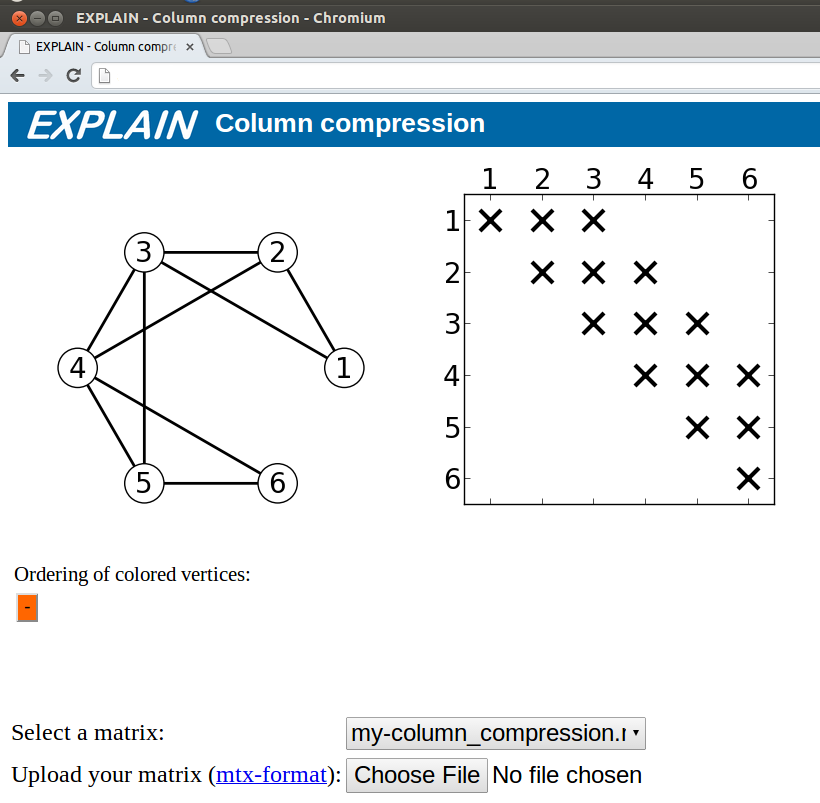
\includegraphics[width=0.5\textwidth]{fig1.png}
\caption{The initial layout of EXPLAIN for some given column compression problem. Matrix and graph are visualized side by side to recognize the underlying connection between these two equivalent representations. Nonzero elements are indicated by the symbol $\times$.
}
\label{fig1}
\end{figure}
We now describe the extension of \mbox{EXPLAIN} by a novel educational module illustrating column compression. The module allows to select and, thus, color the vertices of a given graph step by step. The order in which the vertices are colored is interactively selected by the student. In each step, when the student selects a vertex, the program checks all of its neighbors regarding the colors. A color of the current step is then greedily selected from a predefined list, $\{1=\text{green}, 2=\text{turquoise}, 3=\text{orange}, 4=\text{violet}, 5=\text{red}, 6=\text{yellow}, ...\}$, such that it differs from the colors of those neighbors that are already colored. Recall that a group of columns corresponds to a set of vertices in the graph with the same color. To indicate this, we do not color only the vertices in the graph but also the corresponding columns in the matrix.

\figurename~\ref{fig1} shows a screenshot of the column compression module. The nonzero elements of the matrix are denoted by the symbol $\times$ in the matrix view; the corresponding column intersection graph is given immediately next to the matrix. In the bottom of the page, different preloaded matrices can be selected or a new matrix can be uploaded from a file on the file system of the student's computer. The tool provides an interactive interface for the student who can control the algorithm such as returning to previous steps or loading different graphs and matrices. Selecting the vertices in different orderings generates different colorings corresponding to different column compressions.

Suppose a vertex is selected in the first step. This vertex is then colored using the first color of the predefined list. Continuing this process of vertex selection, different colors are chosen and an ordered list of vertices is created which is already indicated in \figurename~\ref{fig1} marked by ''Ordering of colored vertices.'' In this figure the list is empty but it will become nonempty in later figures. Each button of this list is clickable, causing \mbox{EXPLAIN} to return back to that step of the algorithm. The process is continued until all vertices are colored. The button labeled by the minus sign, will return to the first step keeping the whole process history.


\begin{figure}
\centering
\subfigure[Student selected $v_2$ and $v_6$ in that order.]{
    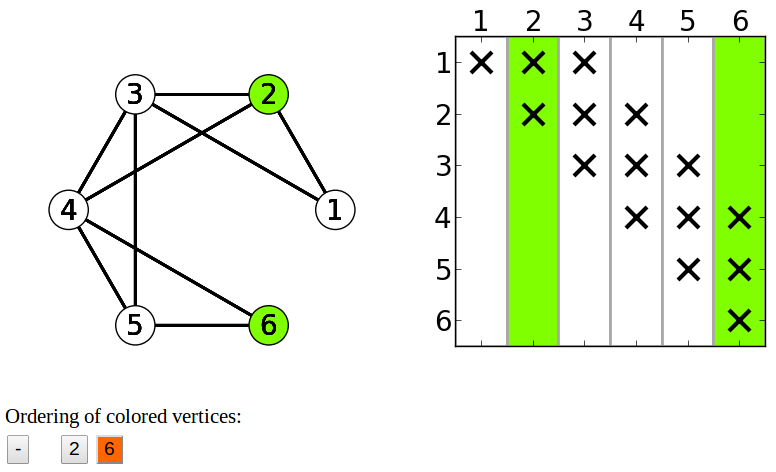
\includegraphics[width=0.47\textwidth]{fig2.png}
    \label{fig2}
}
\centering
\subfigure[Student selected $v_2$, $v_6$, $v_3$, $v_5$, $v_1$, and $v_4$ in that order.]{
    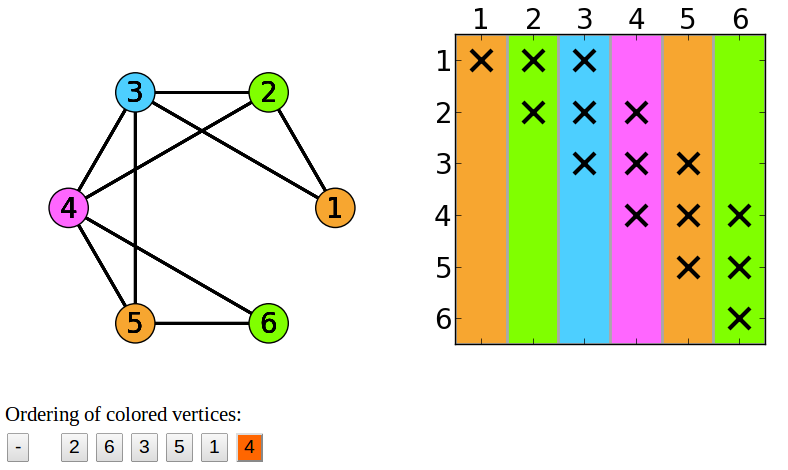
\includegraphics[width=0.47\textwidth]{fig3.png}
    \label{fig3}
}
\centering
\subfigure[Student selected vertices as in \figurename~\protect\ref{fig3} and then jumped back to $v_2$.]{
    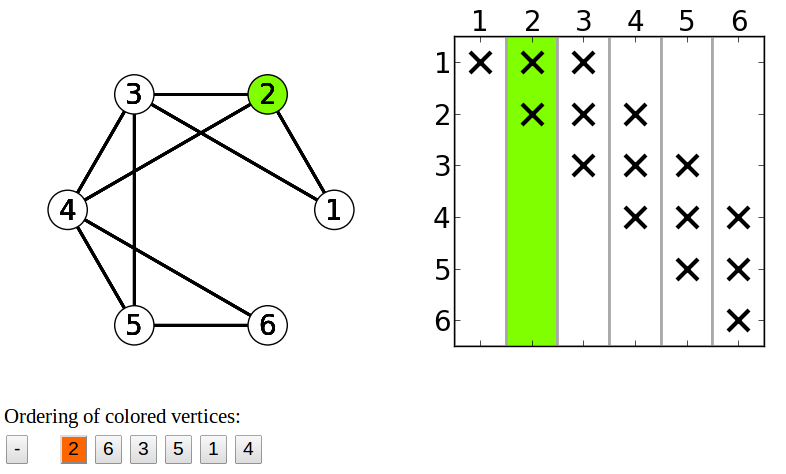
\includegraphics[width=0.47\textwidth]{fig4.png}
    \label{fig4}
}
\centering
\subfigure[Student selected $v_2$, $v_1$, $v_3$, $v_4$, $v_5$, and $v_6$ in that order.]{
    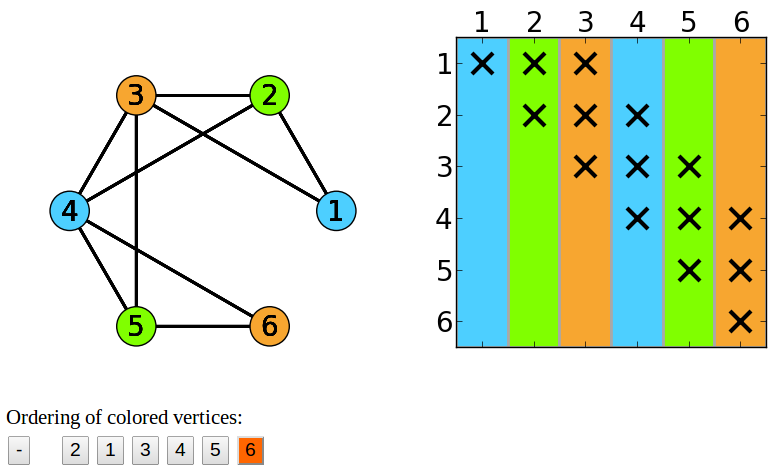
\includegraphics[width=0.47\textwidth]{fig5.png}
    \label{fig5}
}
\caption{Display of various situations after interactively choosing vertices.}
\label{algorihtm}
\end{figure}
\figurename~\ref{fig2} shows a representation of nonzero pattern of the possible following matrix 
\begin{equation}
\label{e:matrixJ}
J =
 \begin{bmatrix}
 1  & 2 & 3 & 0 & 0 & 0 \\
 0  & 4 & 5 & 6 & 0 & 0 \\
 0  & 0 & 7 & 8 & 9 & 0\\
 0  & 0 & 0 & 10 & 11 & 12\\
 0  & 0 & 0 & 0 & 13  & 14  \\
 0  & 0 & 0 & 0 & 0 & 15
 \end{bmatrix},
\end{equation} 

and the related graph in which the student has already selected the two vertices $v_2$ and $v_6$. \figurename~\ref{fig3} represents the final step which shows that four colors are needed when the vertices are selected in the order $(v_2, v_6, v_3, v_5, v_1, v_4)$ displayed in the vertex list. The group of columns with the same color is compressed to a single column in the seed matrix as follows,
\begin{equation}
\label{e:matrixS}
J \cdot S =
J \cdot
 \begin{bmatrix}
 0  & 0 & 1 & 0 \\
 1  & 0 & 0 & 0 \\
 0  & 1 & 0 & 0 \\
 0  & 0 & 0 & 1 \\
 0  & 0 & 1 & 0 \\
 1  & 0 & 0 & 0
 \end{bmatrix}
=
 \begin{bmatrix}
 2  & 3 & 1  & 0 \\
 4  & 5 & 0  & 6 \\
 0  & 7 & 9  & 8 \\
 12 & 0 & 11 & 10\\
 14 & 0 & 13 & 0 \\
 15 & 0 & 0  & 0
 \end{bmatrix}.
\end{equation}
Furthermore, the coloring of \figurename~\ref{fig3} is exactly the one corresponding to that compressed Jacobian~\eqref{e:matrixS}.

Since we want to provide the possibility to return back to some step of the algorithm, a history of the selection process is kept in the ordered vertex list. Now, suppose the student selects to return back to the step $1$ where the vertex $v_2$ was selected, then the program returns back to that step of the algorithm. The resulting state is depicted in \figurename~\ref{fig4}. Notice that the program keeps the whole history and the student can click on any other vertex in the history.

On the other hand, the student can select a completely new selection order from the current step which can generate a smaller or larger number of colors. Employing the different ordering $(v_2,v_1,v_3,v_4,v_5,v_6)$ shown in \figurename~\ref{fig5} leads to a reduction of one color compared to the first ordering given in \figurename~\ref{fig3}. Actually, this is the minimum number of colors needed to color this graph. The corresponding seed matrix is given by
$$
S =
 \begin{pmatrix}
 1 & 0 & 0 \\
 0 & 1 & 0 \\
 0 & 0 & 1 \\
 1 & 0 & 0 \\
 0 & 1 & 0 \\
 0 & 0 & 1 \\
 \end{pmatrix}.
$$


\section{Bidirectional Compression}
\label{s.bidirectional}
In our publication~\cite{2014:09}, we design and implement an interactive module to
teach bidirectional compression and its connection to star bicoloring.
Figure~\ref{f.explain} shows an overview of the layout of the new module whose top and
bottom part are shown in~(a) and~(b), respectively. In the top part, a graph and a matrix
are visualized next to each other. Here, a matrix with a sparsity pattern in the form of
an arrow is taken as an example. The nonzero pattern of the matrix is shown right and the
corresponding bipartite graph is depicted left. A vertex $r_i$, which is placed on the
left part of the graph, represents the $i$th row of the matrix. Likewise, a vertex on the
right part of the graph labeled $c_i$ corresponds to the $i$th column of the matrix.
Different matrices can be selected from a predefined list or can be uploaded to the
server using the menu depicted in Fig.~\ref{f.explain} (b). We stress that EXPLAIN is
designed for small problem instances.

%------------------------------------------------------------------------------------------------
\begin{figure}
  \centering
  \subfigure[]{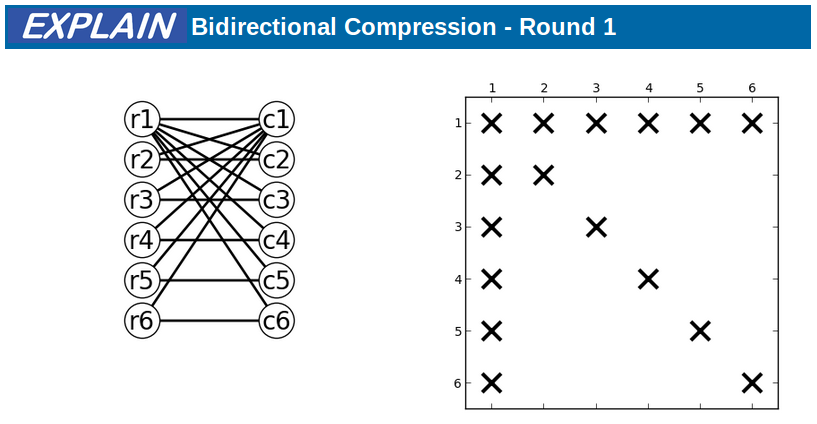
\includegraphics[width=0.43\textwidth]{init-bipartite}}
  \hfill
  \subfigure[]{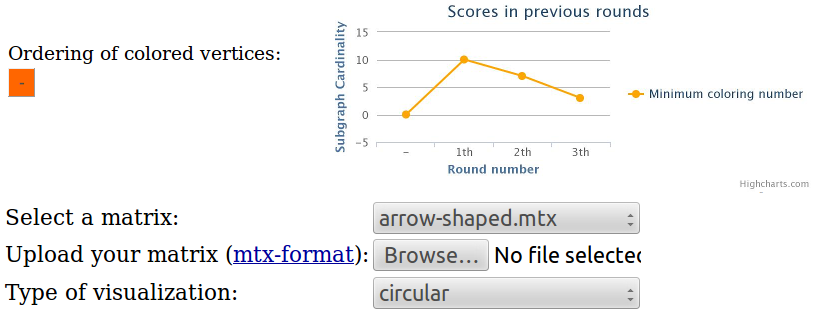
\includegraphics[width=0.55\textwidth]{explain_bottom}}
  \caption{The general layout of the bidirectional compression module. (a) The top part
  contains the visualization of the graph and its corresponding matrix. (b)
   The bottom part contains the intermediate steps, the input, and the
   history of selections.}
  \label{f.explain}
 \end{figure}
%------------------------------------------------------------------------------------------------


%------------------------------------------------------------------------------------------------
\begin{figure}[b]
\centering
\subfigure[]{%
  % Matrix C: after choosing 2 vertices
  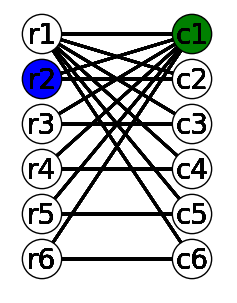
\includegraphics[width=0.18\textwidth]{arrow-shaped-bipartite-graph-twoselected}
  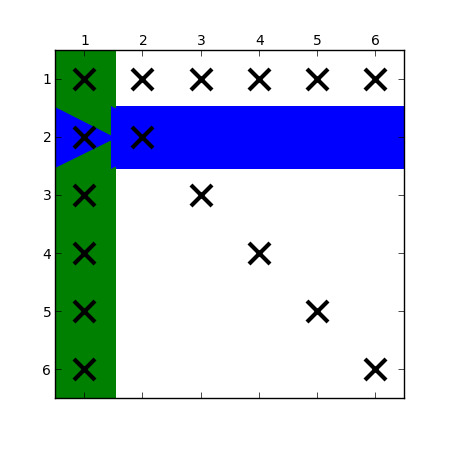
\includegraphics[width=0.24\textwidth]{arrow-shaped-matrix-twoselected}
}
 \hfill
\subfigure[]{%
  % Matrix C: after having completed the solution process
  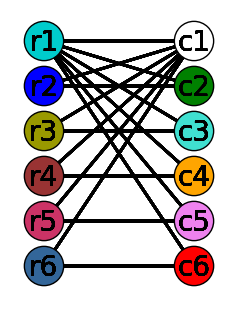
\includegraphics[width=0.18\textwidth]{arrow-shaped-almost-worst-coloring-graph}
  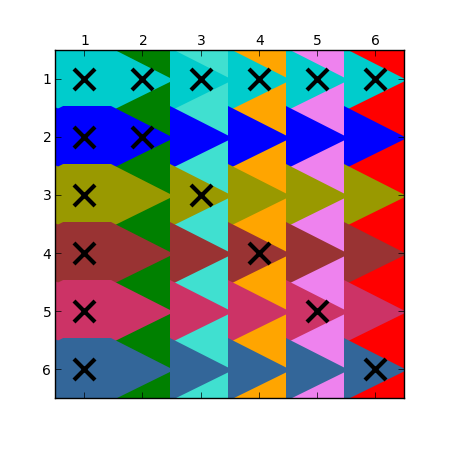
\includegraphics[width=0.24\textwidth]{arrow-shaped-almost-worst-coloring-matrix}
  }%
\caption{The graph and the nonzero pattern (a) taken from Fig.~\protect\ref{f.explain}
after the student interactively selected the vertices $r_2$
and $c_1$. A star bicoloring (b) of that example after trying to solve
\MinStaBic\ interactively. This star bicoloring uses $11$ colors.}
\label{f.arrow-shaped2}
\end{figure}
%------------------------------------------------------------------------------------------------

Using any web browser, the student can interactively solve \MinStaBic\ by clicking on
vertices of the bipartite graph. The selection of a vertex by a click refers to choosing
this vertex to be colored next. This coloring is visualized simultaneously in the graph
as well as in the matrix where the neutral color is the color white. By clicking on a row
vertex, the vertex itself and the corresponding row is colored. This color should obey
the rules specified in the definition of a star bicoloring. By clicking on a column
vertex, this vertex and the corresponding column are colored. Recall that a nonzero
element may be in both a colored column as well as in a colored row. In this case, we
divide the square surrounding this element into a triangle and the remaining part. The
triangle part is colored with the row color and the remaining part of the rectangle with
the column color.

%------------------------------------------------------------------------------------------------
\begin{figure}
\centering
\subfigure[]{%
  % Matrix C: Minimal number of colors
  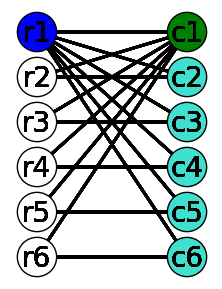
\includegraphics[width=0.18\textwidth]{arrow-shaped-best-coloring-graph}
  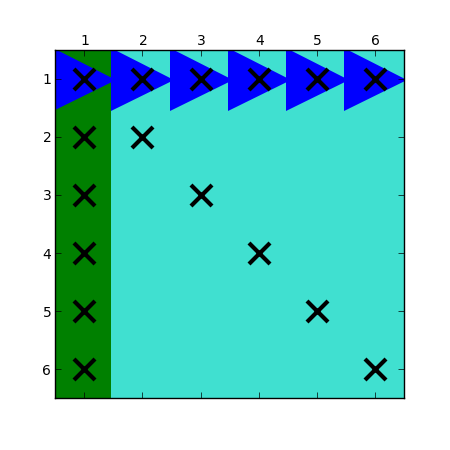
\includegraphics[width=0.24\textwidth]{arrowshaped-best-coloring-matrix}
  }%
  \hfill
\subfigure[]{%
  % A different matrix : after having completed the solution process
  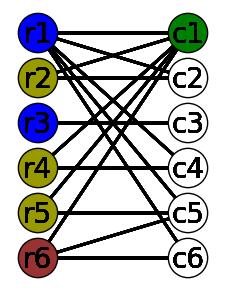
\includegraphics[width=0.18\textwidth]{arrow-shaped2-best-coloring-graph}
  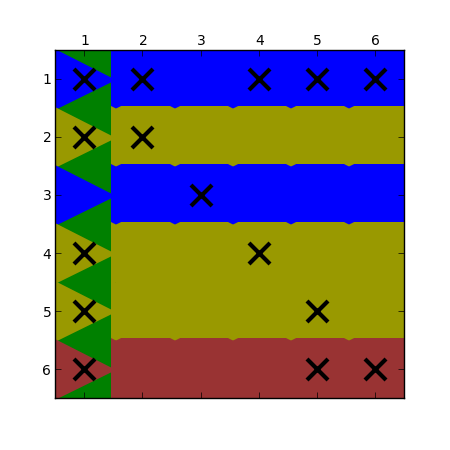
\includegraphics[width=0.24\textwidth]{arrow-shaped2-best-coloring-matrix}
  }%
\caption{A star bicoloring (a) of the problem instance from
Fig.~\protect\ref{f.explain} also considered in Fig.~\protect\ref{f.arrow-shaped2}. This
star bicoloring uses $3$ colors and is an exact solution of \MinStaBic. A star bicoloring
(b) of a different problem instance using $4$ colors which is also an exact
solution of \MinStaBic} \label{f.arrow-shaped4}
\end{figure}
%------------------------------------------------------------------------------------------------

We now take the problem with the arrow-shaped nonzero pattern from Fig.~\ref{f.explain}
as an example. Here and in the following, we zoom into the graph and matrix view of the
layout. The student interactively selects a sequence of row and column vertices to solve
\MinStaBic. Figure \ref{f.arrow-shaped2} (a) shows the situation after the student
selected the vertices $r_2$ and $c_1$.

The interactive selection then goes back and forth until a correct star bicoloring is
found. In EXPLAIN, the process of computing a solution of \MinStaBic\ is called a round.
The current round number is displayed at the top of the web page; see
Fig.~\ref{f.explain}~(a). When a coloring is found at round number $x$, the page shows
the message ``Round $x$ is completed!''

Selecting vertices in different orders will typically result in different star
bicolorings. A star bicoloring which is interactively chosen will not always have a
minimal number of colors. For example, the order of vertex selection visualized in
Fig.~\ref{f.arrow-shaped2}~(b) leads to a star bicoloring using $11$ colors, which is
obviously not the minimal number of colors. Here, all columns and rows are colored
differently. In contrast, Fig.~\ref{f.arrow-shaped4}~(a) illustrates an exact solution of
\MinStaBic\ for this problem instance using the minimal number of $3$ colors.

After completing a round, the student can solve the same problem instance once more. In
this case, the round number will be incremented, the colors will be removed, and another
round is started using the initial situation depicted in Fig.~\ref{f.explain}~(a). The
history of the number of non-neutral colors used in previous rounds is displayed below
the matrix in a score diagram as shown in Fig~\ref{f.explain}~(b). The idea behind this
score diagram is to use elements of game design to motivate and increase the student's
activity in the learning process. This way, the student can see how successful he or she
was in reducing the number of non-neutral colors.

The subtle issues in understanding the connection between bidirectional compression and
star bicoloring are more lucid when considering more irregularly-structured nonzero
patterns. Another problem instance with a different nonzero pattern is shown in
Fig.~\ref{f.arrow-shaped4}~(b). Here, it is more difficult to find out that this star
bicoloring with $4$ colors is indeed an exact solution to \MinStaBic.

\section{Partial Jacobian Computation}

\section{Nested Dissection Ordering}
\subsection{Bisection}
\cite{2014:02}
\begin{figure}
\centering
\subfigure{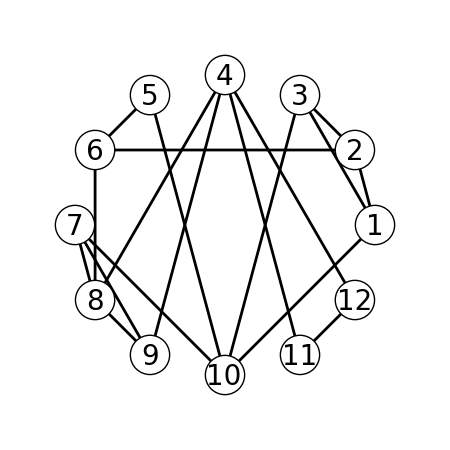
\includegraphics[width=0.48\textwidth]{graph_initial}}%
\subfigure{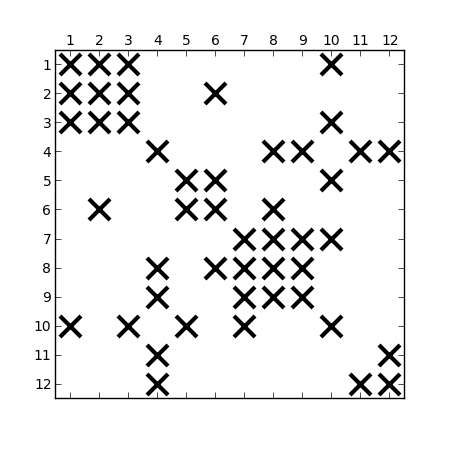
\includegraphics[width=0.48\textwidth]{matrix_initial}}
\caption{Two equivalent representations in terms of a graph (left) and a matrix (right).}
\label{initial}
\end{figure}


\begin{figure}
\centering
\subfigure{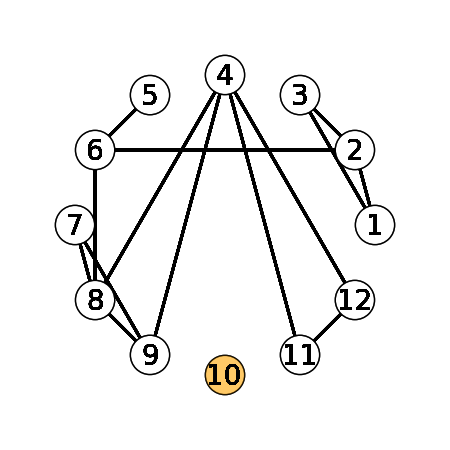
\includegraphics[width=0.48\textwidth]{graph_10_selected}}%
\subfigure{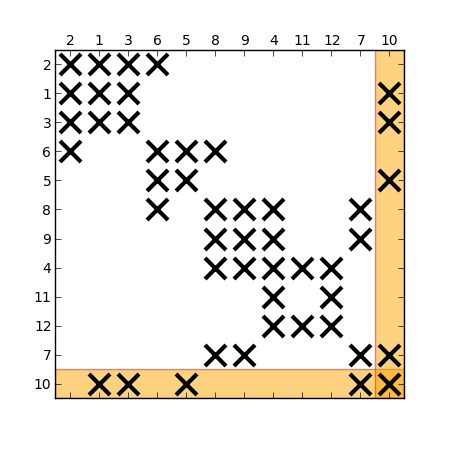
\includegraphics[width=0.48\textwidth]{matrix_10_selected}}
\caption{Graph and matrix view after selecting the vertex number~10. The decomposition into two blocks is still not shown as the graph is not yet decomposed into two disconnected components.}
\label{selected10}
\end{figure}


\begin{figure}
\centering
\subfigure{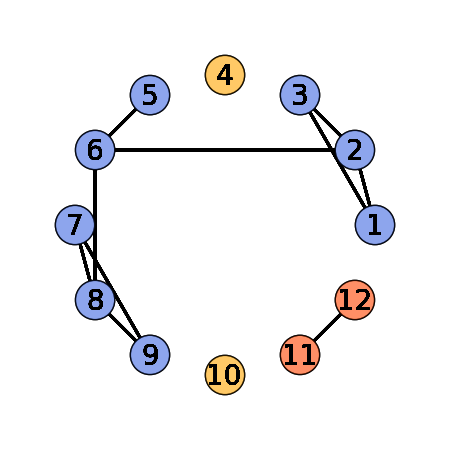
\includegraphics[width=0.48\textwidth]{graph_4_10_selected}}%
\subfigure{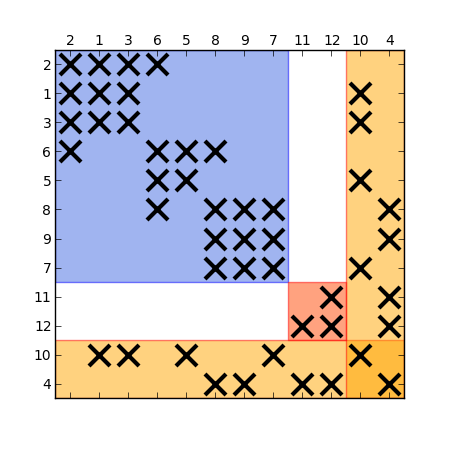
\includegraphics[width=0.48\textwidth]{matrix_4_10_selected}}
\caption{Graph and matrix view after selecting the vertices number 10 and then 4. The selection is not adequate as the sizes of blocks are not balanced.}
\label{selected410}
\end{figure}


\begin{figure}
\centering
\subfigure{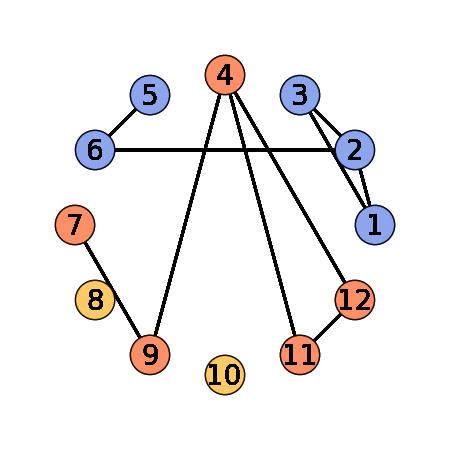
\includegraphics[width=0.48\textwidth]{graph_8_10_selected}}%
\subfigure{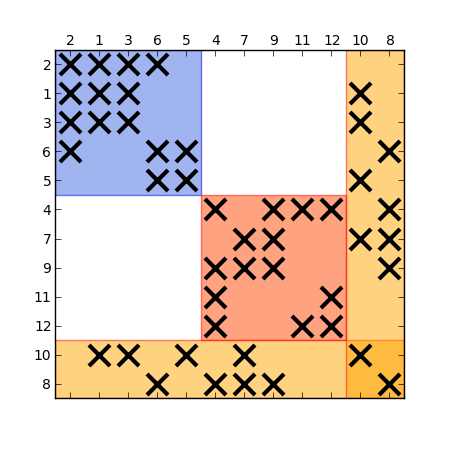
\includegraphics[width=0.48\textwidth]{matrix_8_10_selected}}
\caption{Graph and matrix view after selecting the vertices number 10 and then 8. The block sizes are balanced and the separator size is minimized.}
\label{selected810}
\end{figure}

\begin{figure}
\centering
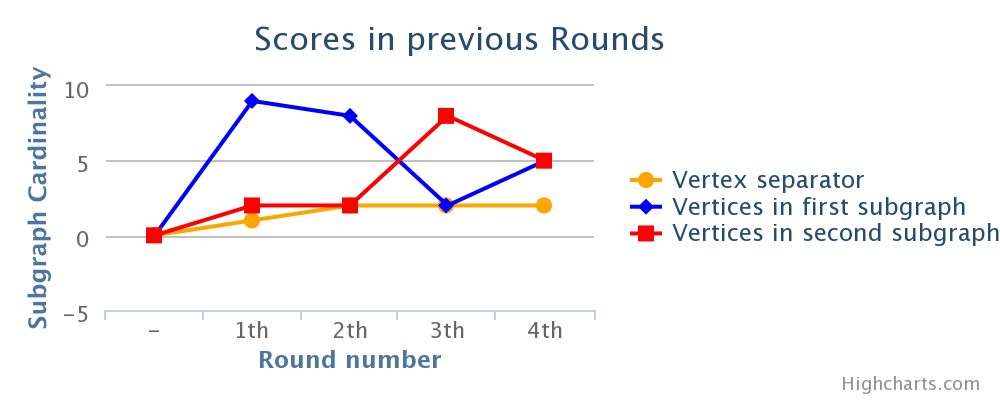
\includegraphics[width=0.47\textwidth]{diagram}
\caption{Score diagram resulting from four different rounds.}
\label{diagram}
\end{figure}

\subsection{Recursive Disection}
\begin{figure}
\centering
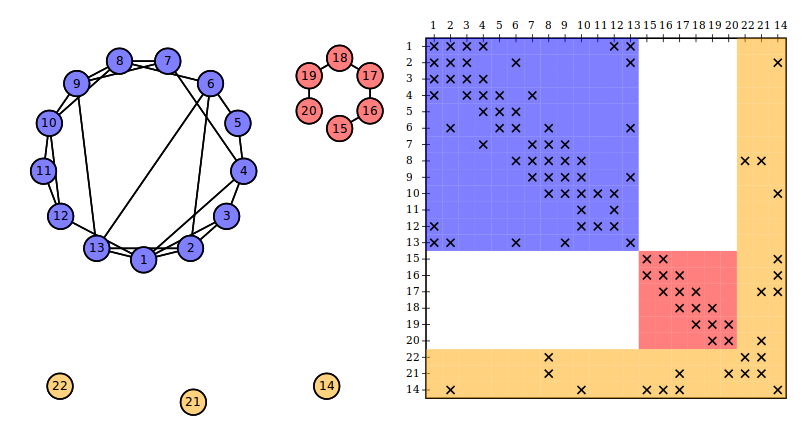
\includegraphics[width=0.47\textwidth]{bad_bisection}
\caption{}
\label{bad_bisection}
\end{figure}

\begin{figure}
\centering
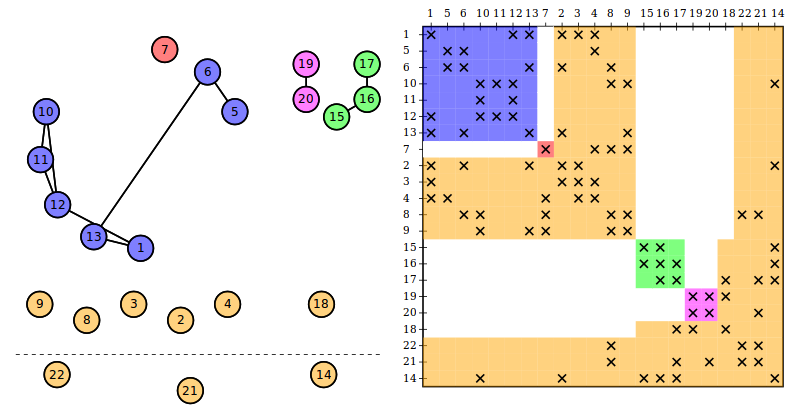
\includegraphics[width=0.47\textwidth]{bad_disection}
\caption{}
\label{bad_disection}
\end{figure}

\begin{figure}
\centering
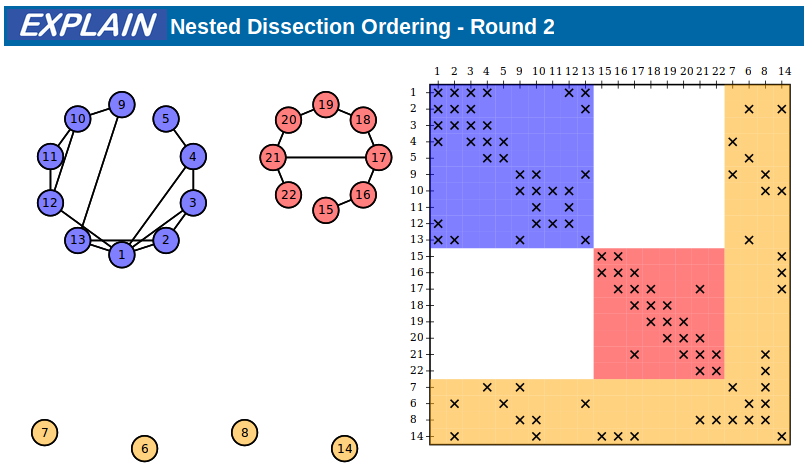
\includegraphics[width=0.47\textwidth]{good_bisection}
\caption{}
\label{good_bisection}
\end{figure}

\begin{figure}
\centering
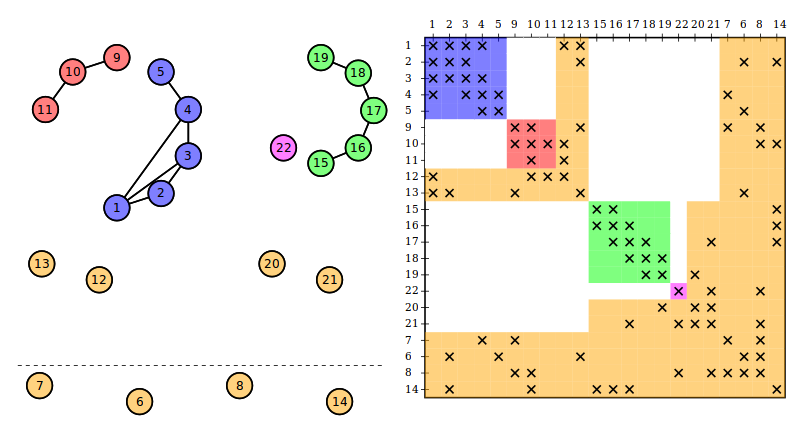
\includegraphics[width=0.47\textwidth]{good_disection}
\caption{}
\label{good_disection}
\end{figure}

\begin{figure}
\centering
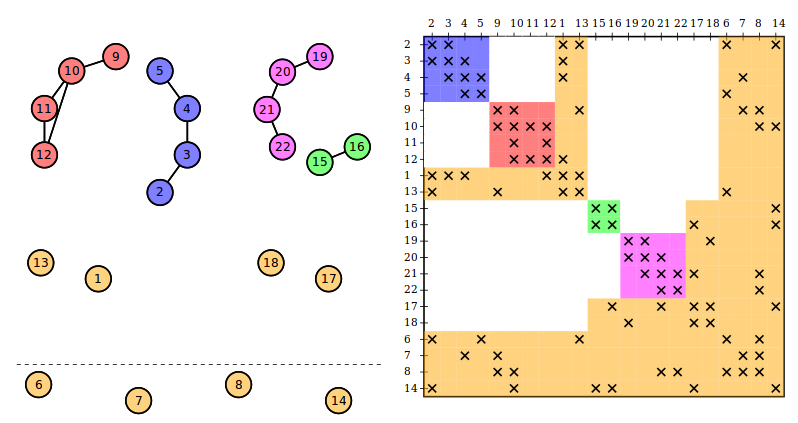
\includegraphics[width=0.47\textwidth]{good_disection2}
\caption{}
\label{good_disection2}
\end{figure}


\begin{figure}
\centering
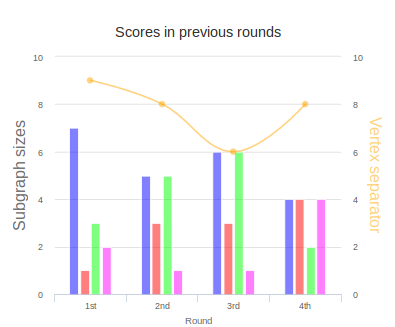
\includegraphics[width=0.47\textwidth]{chart2}
\caption{}
\label{barchart}
\end{figure}

\section{Parallel Matrix Vector Product}
\cite{2015:3}
%------------------------------------------------------------------------------------------
% Overall Layout of Module
\begin{figure}
\centering
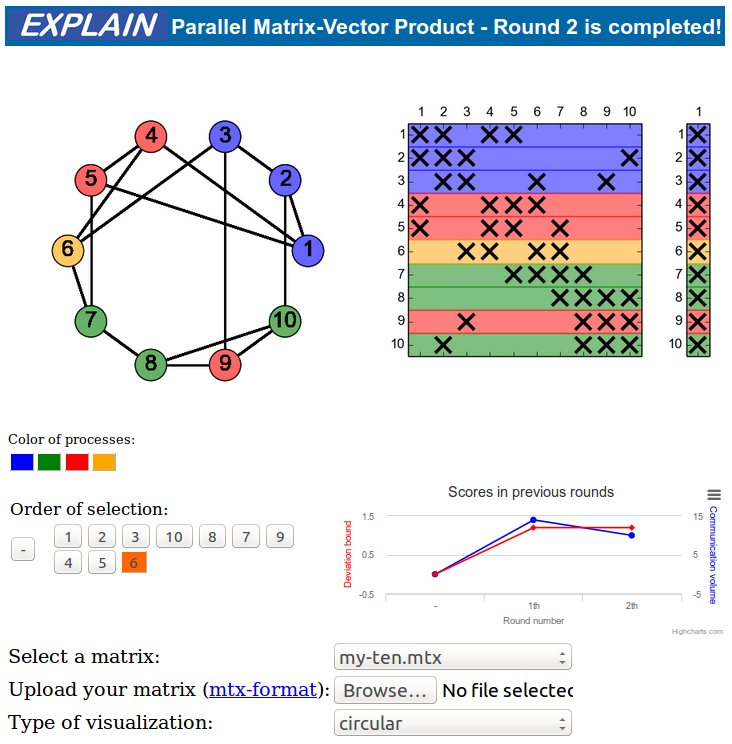
\includegraphics[width=0.9\textwidth]{final}
\caption{Overall structure of the sparse matrix-vector multiplication module.}
\label{f.explain2}
\end{figure}
%------------------------------------------------------------------------------------------

%------------------------------------------------------------------------------------------
% Interactive Selection of Vertices
\begin{figure}
\centering
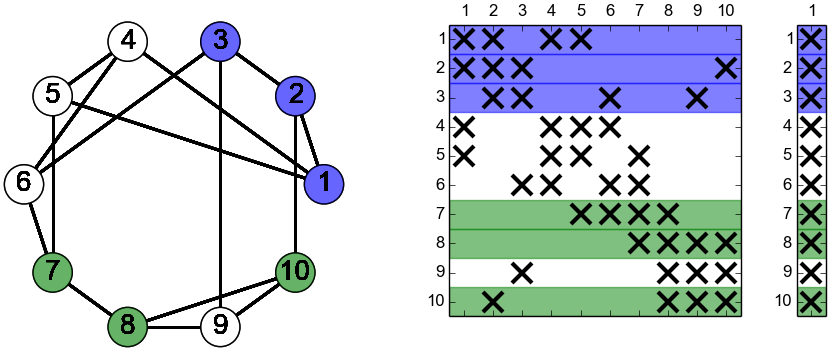
\includegraphics[width=0.9\textwidth]{twoColors}
\caption{The intermediate state after the student selected six vertices.}
\label{f.beginning}
\end{figure}
%------------------------------------------------------------------------------------------

%------------------------------------------------------------------------------------------
% Communication structure
\begin{figure}
\centering
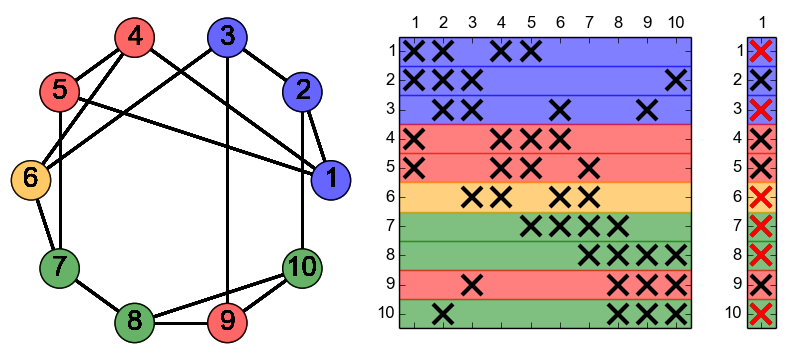
\includegraphics[width=0.9\textwidth]{redComm}
\caption{All vector entries $x_i$ to be communicated to the red process are drawn in red.}
\label{f.communication}
\end{figure}
%------------------------------------------------------------------------------------------

%------------------------------------------------------------------------------------------
% Score diagram
\begin{figure}
\centering
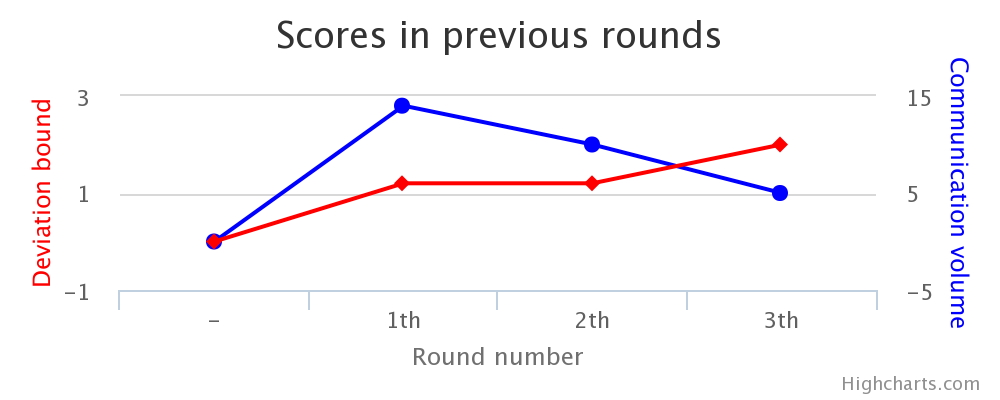
\includegraphics[width=0.8\textwidth]{chart}
\caption{The communication volume and the deviation bound versus various rounds.}
\label{f.score}
\end{figure}
%------------------------------------------------------------------------------------------

\section{EXPLAIN Revisited}
We improved the software EXPLAIN in two ways. 
First, we speed up the software by changing the backbone implementation
which the details is found in Chapter~\ref{s.impl.explain}.
Second, we extended EXPLAIN such that the user can add a custom module 
in an easy scripting lanugage. The program can be written directly 
in the third frame shown beside the matrix and graph frames
(see Figure~\ref{f.custom}).

%------------------------------------------------------------------------------------------
% Score diagram
\begin{figure}
\centering
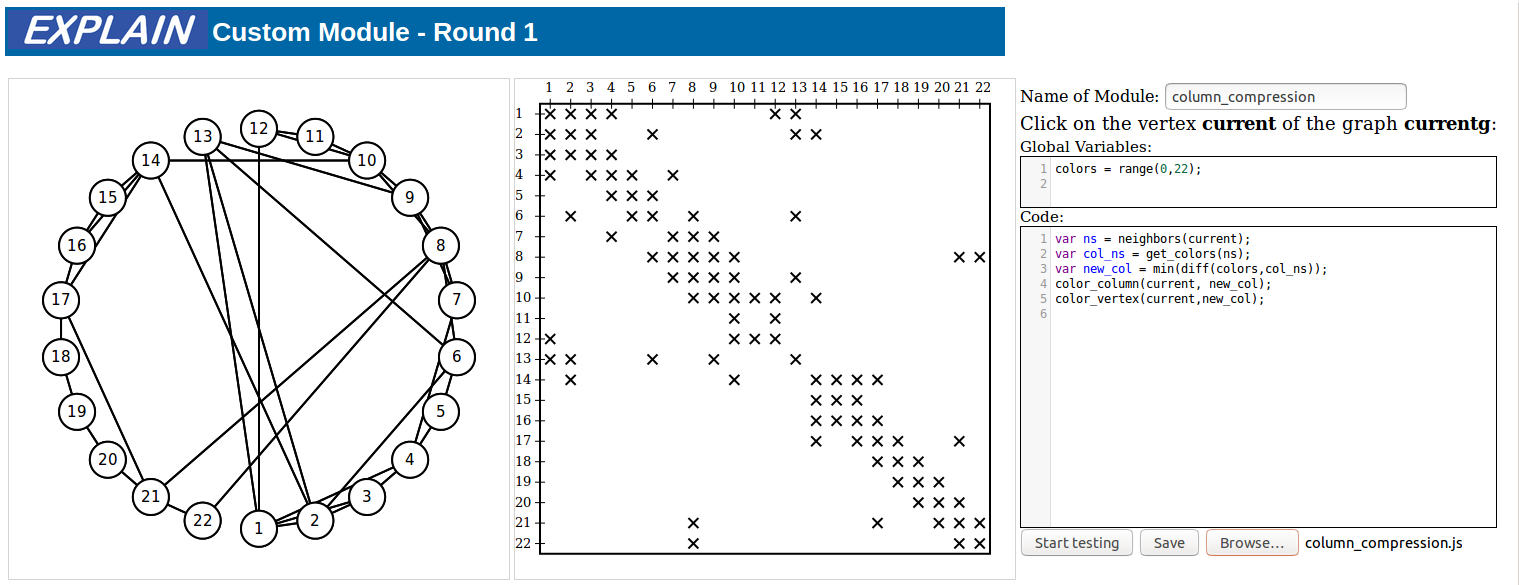
\includegraphics[width=0.98\textwidth]{custom}
\caption{}
\label{f.custom}
\end{figure}
%------------------------------------------------------------------------------------------

\chapter{Computational Package for Coloring and Preconditioning}
\label{package}
\section{Colorings for Full and Partial Jacobian Computation}
\section{Preconditioning}
\section{GraphTea}
Michael Luelfesmann was developed a software which computes a small set of 
coloring and preconditioning. We improved the software regarding the algorithms
and the visualizations. Specially, the user can select different orders for two heuristics
which we discussed before.
For this purpose, we extend GraphTea~
\cite{2014:07,2014:15,2014:16,2015:05,2015:06,2015:07,2015:08} to have a
set of reports for graph coloring. We
%Chemical Graph theory\cite{2015:05,2015:06,2015:07,2015:08}
GraphTea is a graph editing framework designed specifically to compute and visualize
different parameters of graphs interactively.
Figure~\ref{f.graphtea} shows a snapshot of the main
graph window together with two additional windows that give more details on the solution
of different graph problems. These separate windows providing additional information are
called ``reports.''

%-----------------------------------------------------------------------------------------------
\begin{figure}
\centering
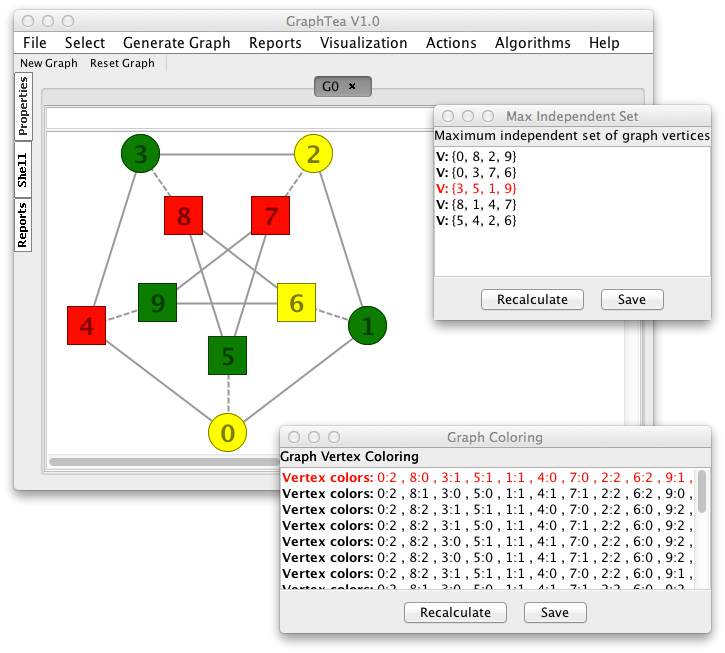
\includegraphics[width=0.7\textwidth]{graphtea}
\caption{An overview of GraphTea: A graph drawing window and 
two floating dialogs with reports on a given graph.}
\label{f.graphtea}
\end{figure}
%-----------------------------------------------------------------------------------------------

\begin{figure}
\centering
   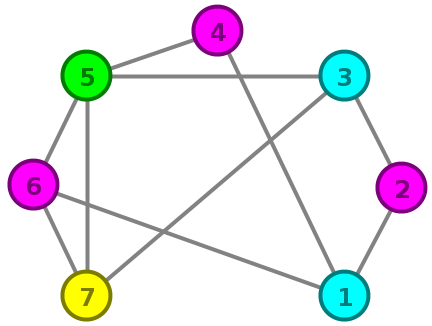
\includegraphics[width=0.45\linewidth]{bad_order_color}
   \hfill
   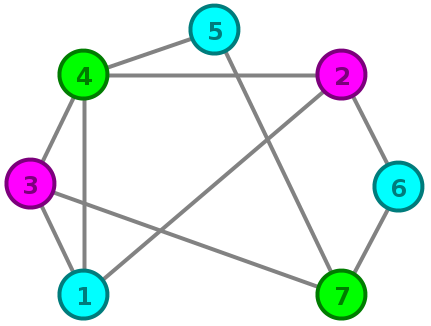
\includegraphics[width=0.45\linewidth]{good_order_color}
\end{figure}


\begin{figure}
\centering
   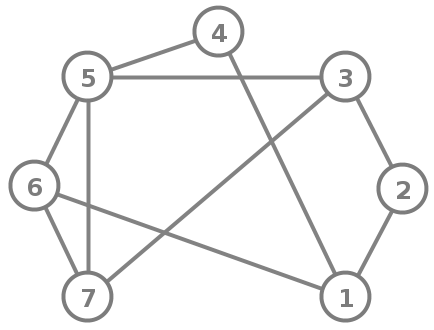
\includegraphics[width=0.4\linewidth]{bad_order}
   \hfill
   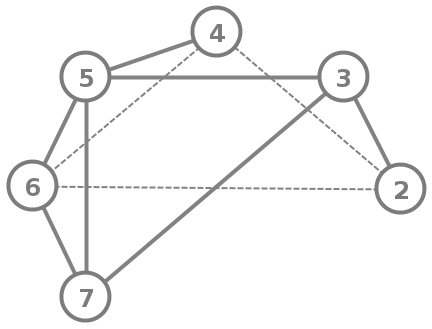
\includegraphics[width=0.4\linewidth]{bad_order_1_removed}
   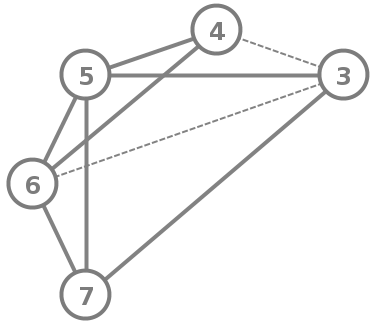
\includegraphics[width=0.4\linewidth]{bad_order_2_1_removed}
   \hfill
   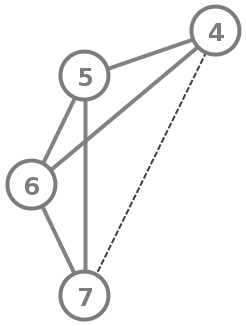
\includegraphics[width=0.3\linewidth]{bad_order_3_2_1_removed}
\caption{The bad  ordering}
\label{bad_order_fillin}
\end{figure}


\begin{figure}
\centering
   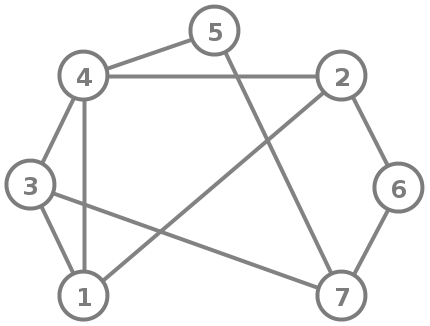
\includegraphics[width=0.4\linewidth]{good_order}
   \hfill
   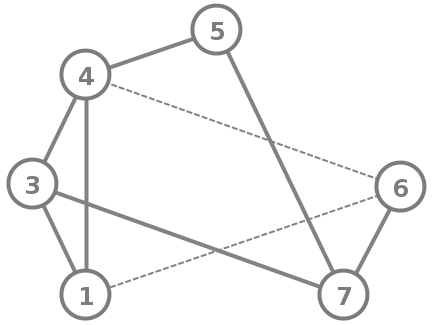
\includegraphics[width=0.4\linewidth]{good_order_2_removed}
   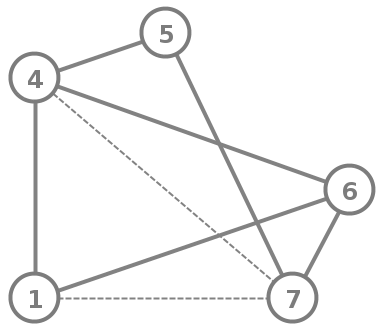
\includegraphics[width=0.4\linewidth]{good_order_3_2}
   \hfill
   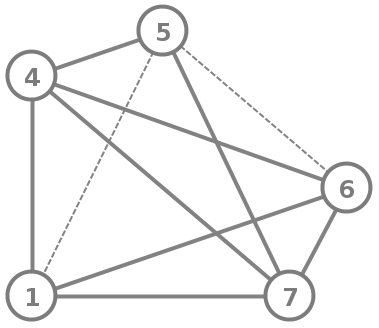
\includegraphics[width=0.4\linewidth]{good_order_4_3_2}
\caption{The good  ordering}
\label{good_order_fillin}
\end{figure}


\begin{figure}
\centering
   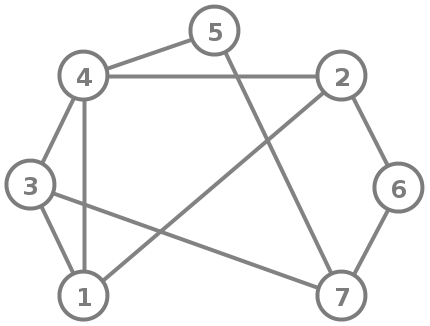
\includegraphics[width=0.4\linewidth]{good_order}
   \hfill
   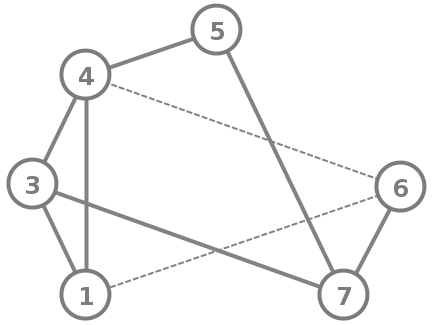
\includegraphics[width=0.4\linewidth]{good_order_2_removed}
   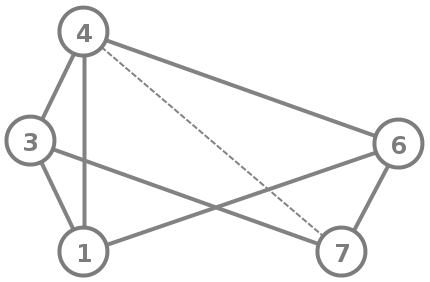
\includegraphics[width=0.4\linewidth]{good_order_5_2_removed}
   \hfill
   \includegraphics[width=0.25\linewidth]{good_order_3_5_2_removed}
\caption{The good  ordering}
\label{good_order_fillin2}
\end{figure}


\chapter{Implementation Details}
\label{impl}
\section{EXPLAIN 1.0}
\label{s.impl.explain}
The previous version of the software \cite{Lulfesmann2010} needed a client with administrator privileges to install Python libraries as well as the software itself. In the new implementation, the software is moved to the online platform which means the student needs just a web browser to work with the software. In this section, we shortly describe the underlying algorithm as well as how it is implemented.

The underlying algorithm of coloring and keeping the history is shown in the pseudo-codes given in \figurename~\ref{f:alg}. The first procedure represents what happens when a student clicks on a vertex. The second one shows how the history of matrix and graph images are loaded when the student clicks on one of the history buttons.

The first procedure, \textsc{VertexClicked}, takes the selected vertex $v$ as an input parameter. To color this vertex $v$, it finds the first color from the list $ColorList$ that is different from the colors of the neighbors of $v$. The coloring of the graph is then changed, shown, and saved as an image. In addition, the vertex $v$ is added to the ordered list, $Hist$, of selected vertices for the history.

The second procedure, \textsc{HistClicked}, takes the selected history $h$. This history will be used to find and plot the previously stored images of the matrix and the graph. Also, the variable $IsInHist$ specifies that the program is in the ``history mode'' which is important if the user selects a vertex different from the previous order. In this case, the program overwrites the existing history and new images will be saved.

\begin{figure}
\centering
\begin{algorithmic}[1]
\State $ColorList \gets \{\text{green}, \text{turquoise},  \text{orange}, \text{violet}, ...\}$
\State $Hist \gets \{\}$\Comment{History of selected vertices.}
\State $WhereInHist \gets 0$\Comment{Where in history are we?}
\State $IsInHist \gets False$\Comment{Are we in history mode?}
\State
\Procedure{VertexClicked}{$v$}\Comment{User clicks vertex $v$.}
\State $ns\gets$  neighbors($v$)
\State $ColorIndex \gets 1$\Comment{Allowed color index}
\For{$i \gets 1$ \textbf{to} size$(ColorList)$}
\State $AllowedColor \gets True$
\For{$j \gets 1$ \textbf{to} size$(ns)$}
\If{$ColorList[i] =$ color$(ns[j])$}
\State $AllowedColor \gets False$
\EndIf
\EndFor
\If{$AllowedColor = True$}
\State $ColorIndex \gets i$
\State Break
\EndIf
\EndFor
\State Color $v$ with the color $ColorList[ColorIndex]$
\State
\If{graph and matrix images are not already saved}
\State SaveMatrix()\Comment{Using a specific name}
\State SaveGraph()\Comment{Using a specific name}
\EndIf
\If{$IsInHist = True$}
\For{$i\gets WhereInHist+1$ \textbf{to} size($Hist$)}
\State $Hist.removeElementAtPosition(i)$
\EndFor
\State $Hist$.add($v$)
\State $IsInHist \gets False$
\Else
\State $Hist$.add($v$)
\EndIf
\State Update($Hist$)\Comment Update history buttons
\EndProcedure
\State
\State
\Procedure{HistClicked}{$h$}\Comment{User clicks history $h$.}
\State OpenMatrix($h$)\Comment{Plot/load matrix with specific name}
\State OpenGraph($h$)\Comment{Plot/load graph with specific name}
\State $WhereInHist \gets find(Hist,h)$\Comment{The location of $h$}
\State $IsInHist \gets True$
\EndProcedure
\end{algorithmic}
\caption{Pseudocode of the event handling in EXPLAIN}
\label{f:alg}
\end{figure}

\mbox{EXPLAIN} combines several Python packages to implement these algorithms. More precisely, the graph data structure is handled by \textit{NetworkX} \cite{networkx2008}. It provides different operations like creation and deletion of vertices and edges. It also allows the programmer to access typical graph information such as the neighbor vertices and the number of vertices. Using this library together with  \textit{matplotlib} \cite{matplotlib2007} covers the different aspects of visualization. Different layouts of graphs as well as the properties of vertices and edges are produced by this library. The matrix manipulation and visualization is handled by \textit{Scipy}~\cite{scipy2001}, specifically the construction and the visual layout of sparse matrices.

The conversion from the standalone to the online version needs the Python library \textit{Mod\_python}~\cite{modpython2013}. It comes from the \textit{Apache} project including the Python interpreter in the given Apache web server. Using this library helps to keep the previous program structure as much as possible.

The library \textit{Mod\_python} assists to implement folder management, user interaction, cookie handling, and the web interface. Specifically, the \textit{Mod\_python} modules like \textit{Apache}, \textit{util}, and \textit{PSession} are used to migrate the previous version of \mbox{EXPLAIN} to a web version. As already mentioned, the Python interpreter is embedded into the web server by the \textit{Mod\_python} module. As a result, the Python code can be run as a web application.

Previously, an event was handled by a local Python function but, in the new version, there are two sides, server and client. The web browser at client side shows HTML websites with embedded  Javascript source code while the server side is written in Python. Since the buttons are HTML buttons and the events are Javascript functions, a form is submitted to the Python server by a Javascript function containing the execution request and parameters to the related Python function. Then, the called Python function writes the dynamically generated result as an HTML string to the Apache request. The server sends back the HTML string and the client shows the string as a web page.

\section{EXPLAIN 2.0}
As we discussed, we changed the code such that it becomes more efficient and easier to extend. 
In the previous version, the module was mainly based on the python libraries:
\textit{NetworkX} \cite{networkx2008} for the graph data structure,
\textit{matplotlib} \cite{matplotlib2007} for the visualization aspects,
\textit{Scipy}~\cite{scipy2001} for the sparse matrix computation, and
\textit{Mod\_python}~\cite{modpython2013} for the web-based version. 

There were two problems with the previous implementation. First, the final visualization
of graph and matrix was always an image. 
So, the time for saving and loading the image was always a problem.
Second, since the final result was HTML/JS code and the computation part was in python,
an overhead of the server management for \textit{Mod\_python} is always added to system.

In the new implementation, we replaced all python parts with the JS code.
We decided for the Javascript library D3 (Data-Driven Documents) 
because of its power of control and visualization.
The adjacnecy list is selected for the graph data structure.
We used the object structure of the JS which helps us to have another
properties also in the graph. Figure~\ref{f.graph-ds} shown an illustration
of the data structure. There is basically an array representing the vertices.
Each cell of array points to another array \textit{edges} which contains
the id numbers of the vertices which are neigbours of that cell.
Here, we showed that the data structure can contain another properties like colors.
It can be extended dynamically to contain any other properties which is needed later.
For example, two other properties \textit{distance} and \textit{parent} are added
in the impelementation of Breadth-First Search (BFS).

%-----------------------------------------------------------------------------------------------
\begin{figure}
\centering
\includegraphics[width=0.38\textwidth]{graph}
\caption{}
\label{f.graph-ds}
\end{figure}
%-----------------------------------------------------------------------------------------------

Another important aspect which is considered in our design was the connection of the 
model and view. An effective approach enables the direct change in view while keeps the 
separation of the view and model. So, we decided to have unique ids for the view of
edges and vertices. The unique ids for vertices are defined as the concatenation of the
string "ver" and the actual id of vertex. Similarly, the unique ids for edges are
defined as the concatenation of the four string "edge", the source vertex, "-", 
and the target vertex. The same idea is used for the matrix view. Each cell of the matrix
is accessible through an unique id combining the strings "cell", the row index,
"-", and the column index. Each nonzero at matrix also gets the unique id same as before 
while inserting the string "nnz" instead of cell.

The previous discussion of the view access enables us to select the 
specific element and change its behaviour and properties. For example, the following 
code would change the color of the vertex with the id~\textit{i} and the color
of a matrix cell,
\begin{lstlisting}
d3.select("ver"+i).set_color(red);
d3.select("cell"+i+"-"+j).set_color(blue);
\end{lstlisting}

There are two important aspects of implementation which we discuss here. 
An aspect of implementation is the real connection of an edge to its
source and target vertices. It means that the locations of the source and target
vertices are read directly from the vertex component in view. This prevents 
of the double repaint the view.
Another aspect is to paint the components in the correct order. So, no edges
are viewed about vertices or no cells of matrix are shown above the nonzeros. 
We did this by using the group component of D3 in which it can be managed
to be drawn always in the given order.

After the first design of the software, we then considered the actual interface
for the developer. Since, we do not need all the functionality which the 
programming language provides, we decided to have a new script language which
has only functionalities regarding the matrix and the graph and their
connections. Also, this new script language does everything by simple functions
such that each function does a specific action on the graph or matrix.
Table~\ref{command-table} shows a list of functions which are availanle
now in EXPLAIN 2.0.
\begin{table}
  \begin{tabular}{ | c | c |}
    \hline
    neighbors($l_v$) & returns the neighbours of the vertex $l_v$  \\ \hline
    color\_vertex($v$,$c$) & colors the vertex $v$ with the color $c$  \\\hline
    color\_column($i$,$c$) & colors the column $i$ with the color $c$  \\\hline
    color\_row($j$,$c$)    & colors the row $j$ with the color $c$  \\\hline
    min($l$) and max($l$) & finds minimum and maximum of the list of integers $l$ \\\hline
    diff($A$,$B$) & finds differenece of two given sets $A$ and $B$ \\\hline
    get\_colors($l_v$) & return a list of colors of vertices $l_v$ \\\hline
\end{tabular}
\caption{The list of functions available in the new scripting language.}
\label{command-table}  
\end{table}

Having such scripting language empowers us to have a dynamic script editor 
together with EXPLAIN which makes the creation of new module very efficient and fast.
The developer of a new module needs only to write the action command of the vertex
click and the global variables which he/she needs.
There are some predefined variables for required data.
As an example, the variable \textit{current} represents the current vertex.
The following code shows the code for the column compression 
module as an instance. The code is very shorter than the implementation in EXPLAIN 1.0.
\begin{lstlisting}
var ns = neighbors(current);
var col_ns = get_colors(ns);
var new_col = min(diff(colors,col_ns));
color_column(current, new_col);
color_vertex(current,new_col);
\end{lstlisting}

\section{Computational Package for coloring}
\label{s.impl.graphtea}
\chapter{Conclusion}
\label{conc}
\bibliographystyle{IEEEtran}
\bibliography{refs}

\end{document}
